\documentclass[10pt]{beamer}
\usetheme{Malmoe}
\setbeamertemplate{navigation symbols}{}
%\colorlet{beamer@blendedblue}{blue!40!black}
\setbeamertemplate{navigation symbols}{}
\newcommand*\oldmacro{}%
\let\oldmacro\insertshorttitle%
\renewcommand*\insertshorttitle{%
\oldmacro\hfill%
\insertframenumber\,/\,\inserttotalframenumber}

\usepackage{caption}
\usepackage{hyperref}
\usepackage[makeroom]{cancel}
\usepackage{ amssymb }
\usepackage{appendixnumberbeamer}
%\usepackage{tikz-feynman}
\usepackage{graphicx}
\begin{document}

\title{Nationwide: Model Risk Management Assessment/Case Study}
\author[Barkeloo]{Jason Barkeloo, Ph.D.}
\date{November 16, 2020}

%\titlegraphic{\includegraphics[width=4cm]{../ATLAS-Logo-Ref-RGB.png}\hspace*{2.75cm}~%
%   \includegraphics[width=4cm]{../uo_logo_green_on_white_2.jpg}
%}

\frame{\titlepage}
\frame{\frametitle{Table of Contents}\tableofcontents[hidesubsections]}

\frame{\frametitle{Code location for further fleshed out examples}

All code for these exercises can be found via this hyperlink as a ipython/jupyter notebook located on my github in addition to attachments sent with the presentation: \\~\\


\hyperlink{https://github.com/JTBarkeloo/JupyterNotebooks/blob/master/MRM Assessment.ipynb}{https://github.com/JTBarkeloo/JupyterNotebooks/blob/master/MRM Assessment.ipynb} 

}

\section{Exploratory Analysis}

\frame{\frametitle{Exploratory Data Analysis}
Summary of 30,000 individuals
\begin{itemize}
\item age - Age of customer
\item inc - Income of customer
\item car - Category of car: Standard, Luxury, Truck
\item edu - Education level of driver (High School or College)
\item acc - Number of accidents over the last two years

\end{itemize}
Want to build a model that will optimize recognition of accident events using these values and attempt to categorize riskier drivers from less risky drivers
Ideal model would have nice bifurcation between classes, difficult to get without more discriminating variables with separation power
Area under ROC curve can be used a a way to classify the model in comparison to other models
%\centering
%\includegraphics[width=0.7\textwidth]{../../ThesisImages/backgrounds.png}
}

\frame{\frametitle{Exploratory Data Analysis}
\begin{itemize}
\item Start by looking at behavior of noncategorical data, Age is oddly uniform
\end{itemize}
\centering
\begin{columns}
\begin{column}{0.5\textwidth}
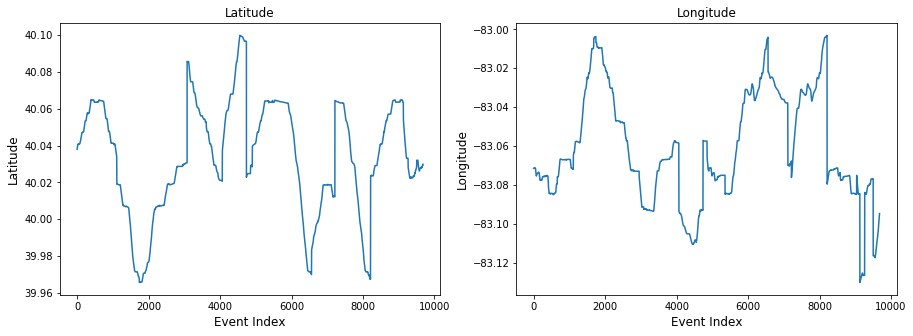
\includegraphics[width=0.9\textwidth]{Images/Image2.png}
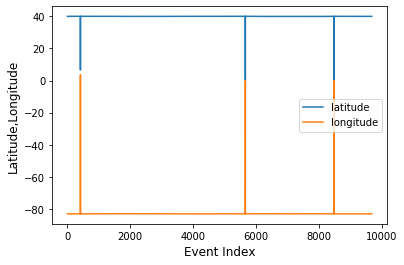
\includegraphics[width=0.9\textwidth]{Images/Image1.png}
\end{column}
\begin{column}{0.5\textwidth}
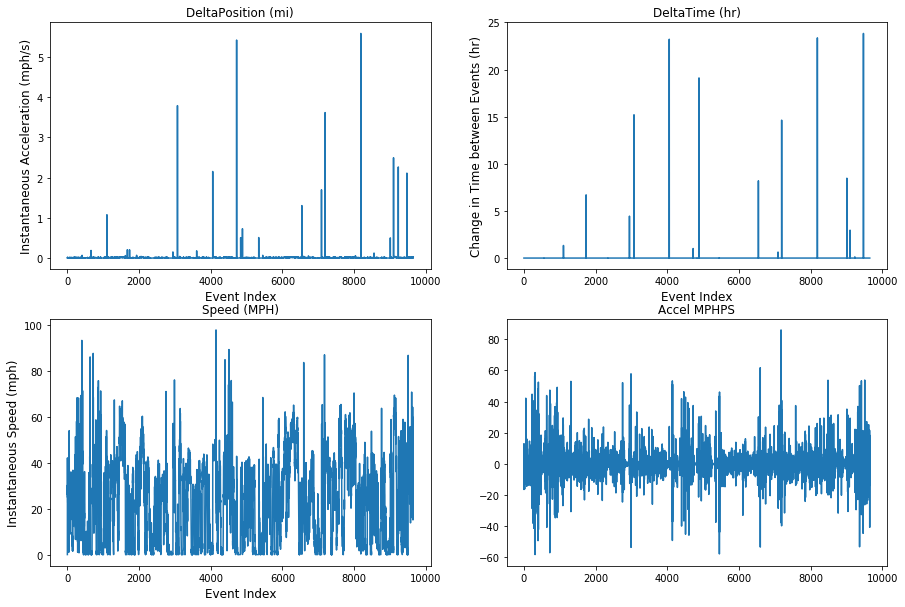
\includegraphics[width=0.8\textwidth]{Images/Image4.png}
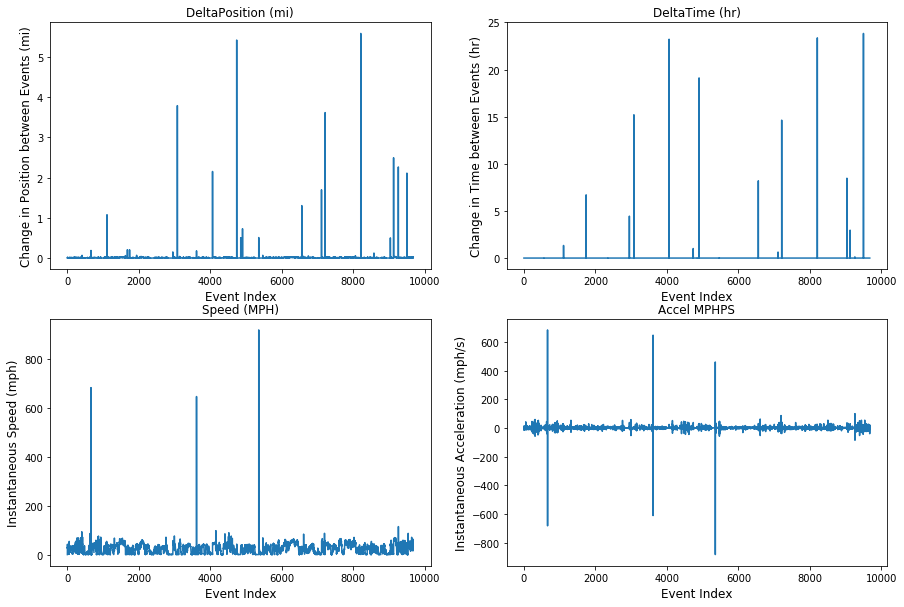
\includegraphics[width=0.9\textwidth]{Images/Image3.png}
\end{column}
\end{columns}
}

%\frame{\frametitle{Further Cleaning - $\Delta$Position, $\Delta$Time, Speed, Acceleration}
%\centering
%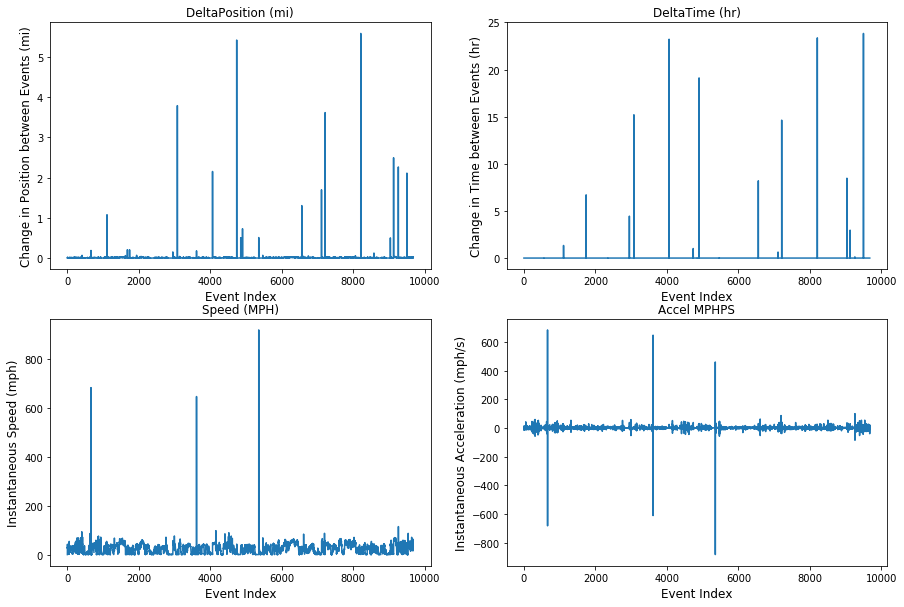
\includegraphics[width=1.\textwidth]{Images/Image3.png}
%}



%%%%%%%%%%%%%%%%%%%%%%%%%%%%%%%%%%%%%%%%%%%%%%%%%%%%%%%%%%%%%%%%%



\frame{\frametitle{Statistical Significance: Vehicle and Education Types}
Z-test used, conclusions to be drawn depend on how liberal the definition of statistical significance being used is \\ 
The use of p$<$0.05 is somewhat arbitrary but is what will be used here as it is a standard choice of convention
\begin{itemize}
\item z value for Standard and Luxury: 3.64
\item z value for Standard and SUV: 5.31 
\item z value for Luxury and Truck: 7.11 
\end{itemize}
The null hypothesis can be rejected for all combinations of Vehicle Types \\
\begin{itemize}
\item z value for High School and College: 0.27
\end{itemize}
The null hypothesis cannot be rejected for Education Type, as such for my models they will be combined and education type not used as a potential discriminator \\~\\
Categorical variables are changed to numbers using one-hot encoding to prevent ranking errors during model building and testing.
}




%%%%%%%%%%%%%%%%%%%%%%%%%%%%%%%%%%%%%%%%%%%%%%%%%%%%%%%%%%%%%%%%%%
\section{Model Building}

\frame{\frametitle{Model Building}
A variety of models were employeed to different ends to try and create a binary classification of risk.  Multiple collision events are classified with single collision events.  With more data a third category of excessive risk could be added to models.  \\~\\
Small minority class, small percentage of those are multiple collision events. \\~\\
Model presented here (with smote oversampling training data):
\begin{itemize}
\item Boosted Decision Tree (BDT) 
\end{itemize}
A training (80\%)/testing(20\%) random set split was done to help ensure unbiased results
%\centering
%\includegraphics[width=0.7\textwidth]{../../ThesisImages/backgrounds.png}
}

\frame{\frametitle{BDT with SMOTE Upsampling}
\begin{itemize}
\item SMOTE Oversampling used to generate synthetic data that is similar to, but not exactly like the minority class, using a nearest-neighbors approach and fills in space between neighbors
\item F Scores can give insight into separation powers of training variables
\item Weight: How frequent splitting occurs on the variable
\item Gain: How useful variable is in terms of separation
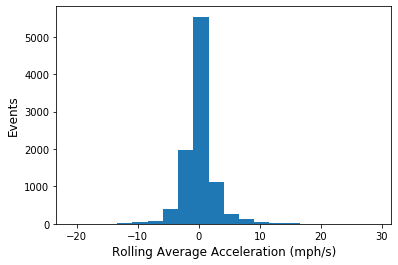
\includegraphics[width=0.9\textwidth]{Images/Image8.png}
\end{itemize}
\begin{columns}
\begin{column}{0.5\textwidth}
%\includegraphics[width=0.9\textwidth]{Images/Image15.png}
\end{column}
\begin{column}{0.5\textwidth}
%\includegraphics[width=0.9\textwidth]{Images/Image16.png}
\end{column}
\end{columns}
}

\frame{\frametitle{BDT with SMOTE Upsampling}
\begin{columns}
\begin{column}{0.5\textwidth}
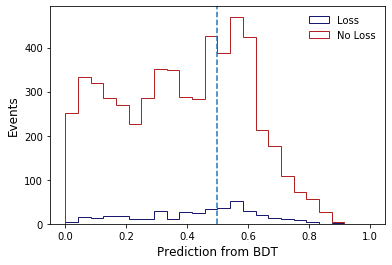
\includegraphics[width=0.9\textwidth]{Images/Image9test.png}

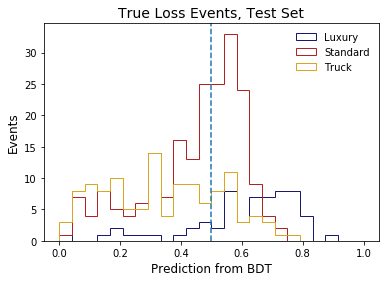
\includegraphics[width=0.9\textwidth]{Images/Image10.png}
\end{column}
\begin{column}{0.5\textwidth}
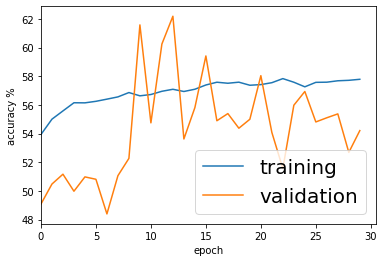
\includegraphics[width=0.9\textwidth]{Images/image13.png}

\includegraphics[width=0.9\textwidth]{Images/Image11.png}
\end{column}
\end{columns}
Balanced Accuracy Score: 0.553
Area Under ROC: 0.55
}

\section{Model Assessment}

\subsection{Model Limitations}
\frame{\frametitle{Model Comments and Limitations}
\begin{itemize}
\item BDT probably overkill with this amount of data/variables, especially given correlations
\item Overtuning difficult to avoid/hyperparameters must be adjusted
\item Samilar result i.e., area under ROC curve as Multivariate Logistic Regression (See Backup)
\item The BDT model over estimates Standard and Luxury loss from no loss cases.  This is most likely do the class makeup that wasnt fully taken into account due to time
\item Essentially the model asserts that cars (both types) are significantly riskier than trucks.  This seems logical as trucks exist in a separate cargo-loading domain as opposed to cars
\item Further data i.e., driving data, would allow this model to be further generalized and the classes further separated
\end{itemize}
}

%\frame{\frametitle{Conclusion}
%\begin{itemize}
%\item Orthogonal validation/control regions are in development
%\end{itemize}
%}


%%%%%%%%%%%%%%%%%%%%%%%%%%%%%%%%%%%%%%%%%%%%%%%%%%%%%%%%%%%%%%%%
%%%%%%%%%%%%%%%%%%%%%%%%%%%%%%%%%%%%%%%%%%%%%%%%%%%%%%%%%%%%%%%% 	
\appendix



\section{Backup}
\frame{\frametitle{Backup}
}

\frame{\frametitle{Multivariate Logistic Regression}
\begin{itemize}
\item Naively we could train a model on the data classes as given
\item With enough separation power i.e., variables distinct enough in each class, this can be used for event classification
\item Balanced Accuracy score: 0.559, Area Under ROC: 0.55
\end{itemize}
\begin{columns}
\begin{column}{0.5\textwidth}
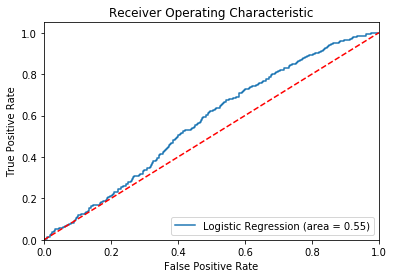
\includegraphics[width=0.9\textwidth]{Images/Image6.png}
\end{column}
\begin{column}{0.5\textwidth}
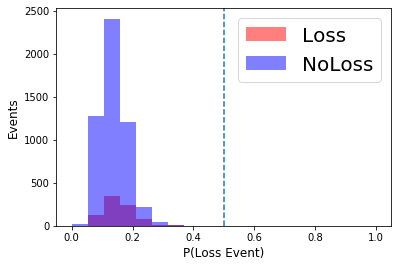
\includegraphics[width=0.9\textwidth]{Images/Image12.png}
\end{column}
\end{columns}
}

\frame{\frametitle{Single Variable Logistic Regression}
\begin{itemize}
\item The simplest model would be to use the highest correlated variable in a single variable logistic regression to classify events
\item Income is highest noncategorical correlated variable to Accidents
\item Balanced Accuracy score: 0.529, Area Under ROC:0.53
\item There is something to be gained including another highly correlated variable (age) here
\end{itemize}
\begin{columns}
\begin{column}{0.5\textwidth}
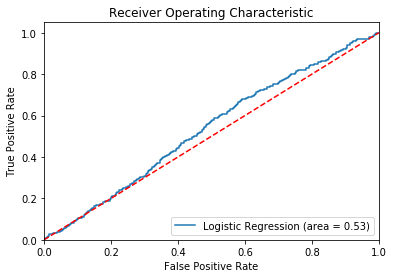
\includegraphics[width=0.9\textwidth]{Images/Image14.png}
\end{column}
\end{columns}
}


\frame{\frametitle{BDT with SMOTE Upsampling}
\begin{columns}
\begin{column}{0.5\textwidth}
Testing Set
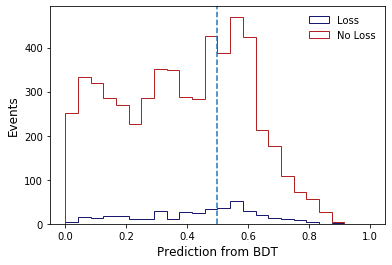
\includegraphics[width=0.85\textwidth]{Images/Image9test.png}

\end{column}
\begin{column}{0.5\textwidth}
Full Set
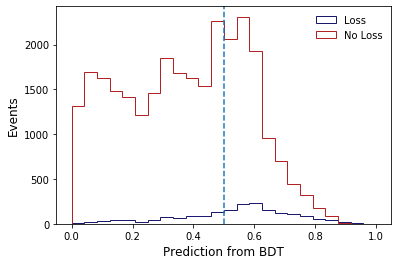
\includegraphics[width=0.85\textwidth]{Images/Image9full.png}

\end{column}
\end{columns}
Balanced Accuracy Score: 0.553
Area Under ROC: 0.55
}

\end{document}

%36.070
